\setchapterpreamble[u]{\margintoc}
\chapter{Cell Annotation}
\labch{cellAnn}

Cell type annotation refers to the process of categorizing and assigning cell types to individual cells based on their gene expression profiles. These annotations are essential for understanding the cellular composition and heterogeneity within a sample, and constitute the basis of all subsequent analyses. Ideally, from the preprocessed data, each label assigned to each cell should be established with the highest possible confidence. However, absolute certainty cannot be achieved for all cell types, as no universal ground truth exists. Even expert human annotations may vary, given that factors such as sex, age, tissue origin, treatment, and disease state can all influence gene expression profiles. Greater specificity in cell annotation translates into a more accurate representation of the biological complexity of the data. It is nonetheless important to acknowledge that cell types are not discrete categories but rather exist along a continuum of states. For example, regulatory T cells (Tregs) represent immature or less specialized versions of CD4+ and CD8+ T cells that have lost expression of the FOXP3 gene. For this reason, gene signatures\sidenote{A \textbf{gene signature} is a curated list of genes that, together, represent a biological identity or state.} must be employed for each cell type that matches the labels of interest.

While QC involves the examination of all cells simultaneously, cell annotation requires the assessment of individual gene expression profiles and their comparison across cells in order to distinguish between cell types. Computational methods have been developed precisely for this purpose; however, result supervision remains essential. Ensuring accurate cell type annotation, even in scRNA-seq data, is a significant challenge, as both expert and automated methods can be biased or constrained by their training data, leading to errors and time-consuming revisions \cite{Wenjin.Ye}. This chapter presents the existing methods for \textbf{Xenium} data cell annotation and describes the approach selected as the final pipeline.

\section{State of the art}

Two broad approaches exist for cell type annotation: supervised and unsupervised methods. While numerous libraries offer algorithms for both, the exploratory process carried out during QC using Seurat and SingleCellExperiment guided the restriction of the analysis to these two frameworks.

\begin{marginfigure}
	\includegraphics{images/AfterpruneScore.png}
	\caption[Visium Example]{Plotting the resulting labels in the tissue is considered a good practice, as cells in nature present an organized structure in tissues. A random stucture of cell types is a clear indicator of wrong labeling. In this picture we have a good annotation of sample DU53. 
	The same tissue can be seen without label coloring in \vrefsec{QC_V} to better appreciate the structural organisation revealed by the annotations.}
\end{marginfigure}

Unsupervised cell annotation methods are particularly relevant when reference datasets are unavailable. They primarily involve clustering scRNA-seq data, followed by manual or automated annotation of the resulting clusters using marker genes. This approach may be sufficient when the gene panel is diverse enough to reliably differentiate between cell types. However, as discussed in \vrefsec{VisiumVSXenium}, the 377 unique genes present in the DUTRENEO clinical trial panel are insufficient to achieve this level of differentiation. As illustrated in \reffig{fig:figure2}, the data lacked the heterogeneity required for unambiguous cell type assignment. Multiple clustering methods were evaluated (Leiden, Louvain, etc.) but all produced mixed clusters, even in the most spatially separated regions of the UMAP\footnote{UMAP and clustering are parallel downstream uses of the same PCA embedding. UMAP renders clustering results interpretable to the human reader but plays no role in computing them. It therefore serves as a sanity check and communication tool rather than as a component of the analytical pipeline.}. Furthermore, unsupervised methods require manual supervision of each resulting cluster per sample, rendering them impractical for large-scale application across all DUTRENEO samples.

\begin{figure}[H]
    \centering
    
\includegraphics[width=\textwidth]{images/STvsSC_Clustering.png} 
    \caption{Illustration of how a limited number of unique genes complicates the analysis. Panel A shows data used in this thesis, generated with a ST technology comprising only 377 unique genes. Panel B, extracted from \href{https://medium.com/@mohamed.y.elsadec_56085/a-comparative-analysis-of-clustering-scrna-seq-data-using-pca-based-and-gnn-driven-approaches-24c9fb8d5ec8}{this blog}, corresponds to single-cell technology data.}
    \labfig{fig:figure2}
\end{figure}

The alternative approach is supervised cell annotation, which involves automated cell type identification using algorithms trained on labelled reference datasets. However, the use of an inappropriate reference dataset can introduce substantial bias into the results. Ideally, a reference dataset specific to the experimental context should be employed; no such dataset was made in the DUTRENEO clinical trial. The complexity is further compounded by the cancer type: muscle-invasive bladder cancer (MIBC) presents a considerably wider variety of cancer cell types compared to, for example, lymphoma, where a small set of genes may be sufficient to distinguish cell types \sidenote{Given that lymphoma predominantly involves tumoral immune cells such as CD4+, CD8+, and B cells}. In MIBC, cancer cell type diversity rules out such a simplified approach.

Xenium gene panels may vary depending on the experiment or instrument used, making it nearly impossible to identify a published study employing the same gene panel, tissue type, and disease condition.  In other words, it is extremely difficult to find a reference dataset you can use, if you do not have a reference made specifically for your sample and protocol. Reference datasets must match the sample in terms of age, sex, tissue, and biological context to be applicable. For these reasons, reference transcriptomes of pure cell types represent a valuable alternative. These are standardized, high-resolution datasets representing the complete set of RNA transcripts produced by specific, purified, or isolated cell populations, effectively serving as molecular fingerprints for particular cell types (e.g., T cells, astrocytes, hepatocytes). They are commonly used to deconvolve mixed bulk RNA-seq data and estimate the proportion of each cell type within a tissue sample. Regarding their applicability to Xenium data, \cite{Jinming Cheng} reports that supervised annotation methods outperform manual approaches for Xenium ST data, and that among all evaluated methods, SingleR\sidenote{SingleR is described in the following section, \vrefsec{Final_CellAnn}.} currently achieves the best performance. This method can be applied using pure cell type transcriptomes even in the absence of a DUTRENEO-specific reference and that is the process made in the DUTRENEO paper. It is important to note, however, that if the reference dataset is of poor quality, manual annotation may be preferable. For this reason, validation of results against marker genes\sidenote{Marker genes are genes whose expression is characteristic of a specific cell type and are used to validate or interpret annotation results. A gene signature is composed of a set of marker or relevant genes.} remains a necessary step in both supervised and unsupervised workflows.

In summary, no universal standard exists for performing cell type annotation; the most appropriate approach depends on the data, experimental protocol, and tissue under study. Given the scale and complexity of the task, several artificial intelligence algorithms have been developed, though few published studies have applied them to MIBC with the level of cell type specificity required by DUTRENEO\sidenote{The cell types used in this analysis were defined prior to the commencement of this thesis, as part of the analysis of pre-treatment samples. Consistency across the full analysis requires the application of the same methodology.}. Traditional probabilistic methods therefore remain predominant. Machine learning approaches such as k-means clustering have also been employed, but tend to fail when distinguishing between closely related cell subtypes, such as CD4+ T cells and Tregs\sidenote{CD4+, CD8+, and Tregs are distinct subtypes of T cells.} which, despite sharing substantial genetic similarity, exhibit sufficient differences to guarantee separation.

\section{Final process}
\labsec{Final_CellAnn}
Cells were annotated using the R package \textbf{SingleR}\cite{Aran.D}, which performs unbiased cell-type identification in single-cell transcriptomic data by comparing each cell against reference transcriptomes of purified cell populations.\sidenote{SingleR is a correlation-based classification algorithm that computes Spearman correlation coefficients using marker genes to assign cell-type labels, followed by a fine-tuning step to improve classification robustness.}

In this study, the \texttt{BlueprintEncodeData} reference dataset was used. To reduce false-positive assignments, the reference was restricted to cell types expected to be present within bladder tumours. The selected reference labels included epithelial cells, fibroblasts, smooth muscle cells, pericytes, neurons, monocytes, CD4 T cells, CD8 T cells, NK cells, B cells, macrophages, endothelial cells, dendritic cells, neutrophils, and eosinophils. The \texttt{SingleR()} function was applied to the raw count matrix using the fine labels of the reference dataset. The final annotation labels included: epithelial cells, fibroblasts, smooth muscle cells, Tregs, monocytes, CD4+ T cells, CD8+ T cells, B cells, NK cells, macrophages, endothelial cells, granulocytes, dendritic cells, and plasma cells.\sidenote{These labels were selected after multiple optimisation trials in order to balance biological specificity with annotation robustness.}

However, as discussed in the previous section, the use of a non-specific reference dataset may introduce substantial bias into the annotation process. Therefore, additional validation steps were incorporated to evaluate the reliability of the SingleR assignments. Cell-type annotations were validated through differential expression (DE) analysis and enrichment analysis.

\begin{figure}[H]
    \centering
    
\includegraphics[width=\textwidth]{images/UMAP_SingleR_DU61.png}
    \caption{UMAP representation of the dataset coloured according to SingleR annotations. The strong intermixing between populations illustrates the difficulty of relying exclusively on unsupervised clustering for cell-type identification.}
\end{figure}

\textbf{Differential expression analysis} is a statistical approach to identify genes whose activity changes between conditions, here our conditions are the distinct cell types. In this context, each annotated cell type was compared against all remaining cells in the dataset in order to identify genes significantly overexpressed within each cluster (i.e. one cell type). This type of analysis tests whether the expression distribution of each gene differs significantly between two groups of cells, using a statistical test with a p-value. The resulting genes are referred to as \textit{marker genes}\sidenote{Marker genes are genes whose expression is characteristic of a specific cell type and are commonly used to validate or interpret annotation results.}. The top marker genes of each cluster were compared against canonical markers expected for the corresponding cell type. For example, if clusters annotated as CD4+ T cells showed expression of its characteristic markers such as \textit{CD4}, \textit{GZMK}, and \textit{IL10}, we can affirm that the results from SingleR for CD4+ T-cells have characteristic expression of their cell type.

\begin{figure}[H]
    \centering
    
\includegraphics[width=\textwidth]{images/dotplot_wide.png}
    \caption{Dot plot showing the top five most highly expressed genes per cell type in a well-differentiated sample. FOXP3 expression is specifically elevated in Tregs and absent in CD4+ and CD8+ T-cell populations, reflecting biologically expected behaviour successfully captured by SingleR. Plasma cells also show strong expression of canonical plasma-cell markers such as TNFRSF17 and MZB1. Although other cell types have highly expressed genes that are neither specific nor canonical to the cell type they come from, they can still be differentiated thanks to other genes. This is proof of biological complexity.}
	\labfig{Dotplot}
\end{figure}

As shown in \reffig{Dotplot}, some genes, such as \textit{PTPRC} or \textit{ACTG2}, are expressed across multiple cell types. This occurs because a gene is considered a marker when its expression is relatively higher in one cluster compared to others, even if it is not exclusively expressed in that cluster. Therefore, differential expression identifies genes that are statistically enriched in a given cluster relative to  the rest of cells NOT in that cluster, but this does not necessarily imply that they are biologically specific determinants of cell identity. In fact, the most differentially expressed genes are not always the ones that best define the biological characteristics of a cell type, as different cell populations may share the same marker genes while expressing them at distinct levels. For this reason, enrichment analysis is essential to provide additional biological context and to identify the pathways and functional processes that more accurately characterize each cell population.

Before proceeding further, it is important to discuss the statistical filtering criteria applied during marker selection. Statistical significance alone (e.g., adjusted \(p-value < 0.05\)) is insufficient because it does not quantify the magnitude of expression differences. For this purpose, the log$_2$ fold change (\(\log_2FC\)) was used. A positive log$_2$ fold change indicates higher expression in the target cluster, whereas a negative value indicates higher expression in the comparison group.

\[
\log_2FC = \log_2\left(\frac{\text{expression in cluster A}}{\text{expression in cluster B}}\right)
\]

Initially, genes were filtered using \(\lvert \log_2FC \rvert > 1\), under the assumption that this would identify highly discriminative markers. However, this introduced a major bias because genes with negative fold changes were also retained, meaning that genes overexpressed in other clusters were incorrectly assigned as markers of the target cluster. This issue particularly affected small or transcriptionally similar populations and produced misleading enrichment signatures, as illustrated in \reffig{AddModuleScoreBAD}.

\begin{figure}[H]
    \centering
    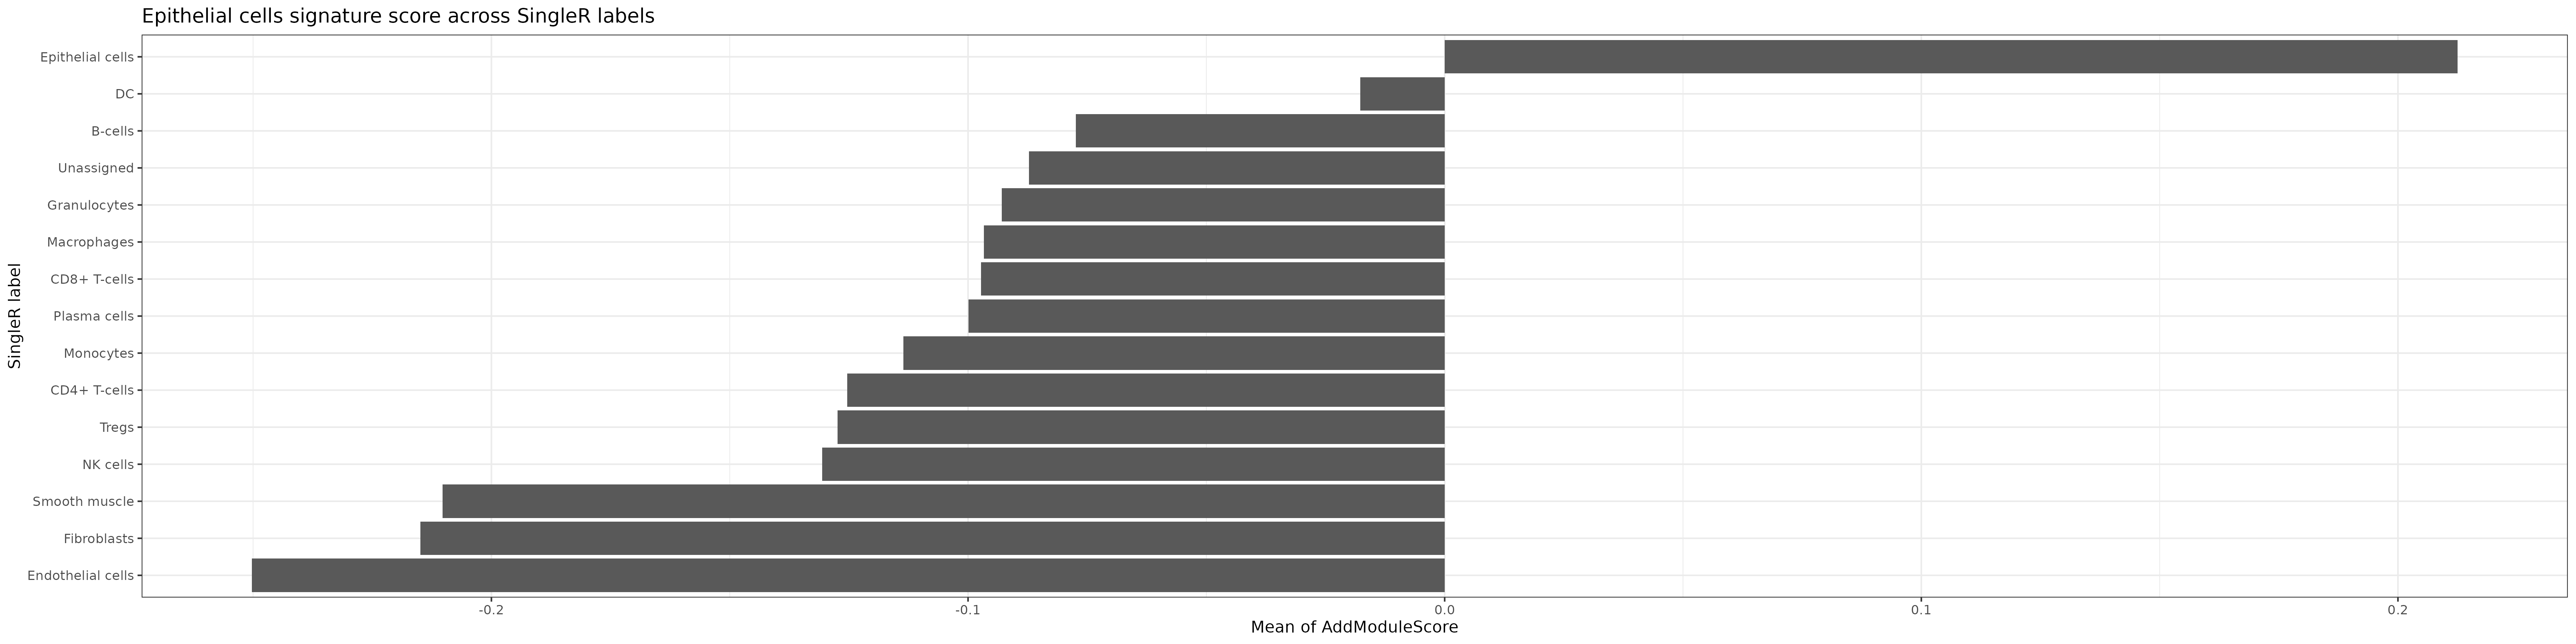
\includegraphics[width=\textwidth]{images/Epithelial_cells_Signature.png}
    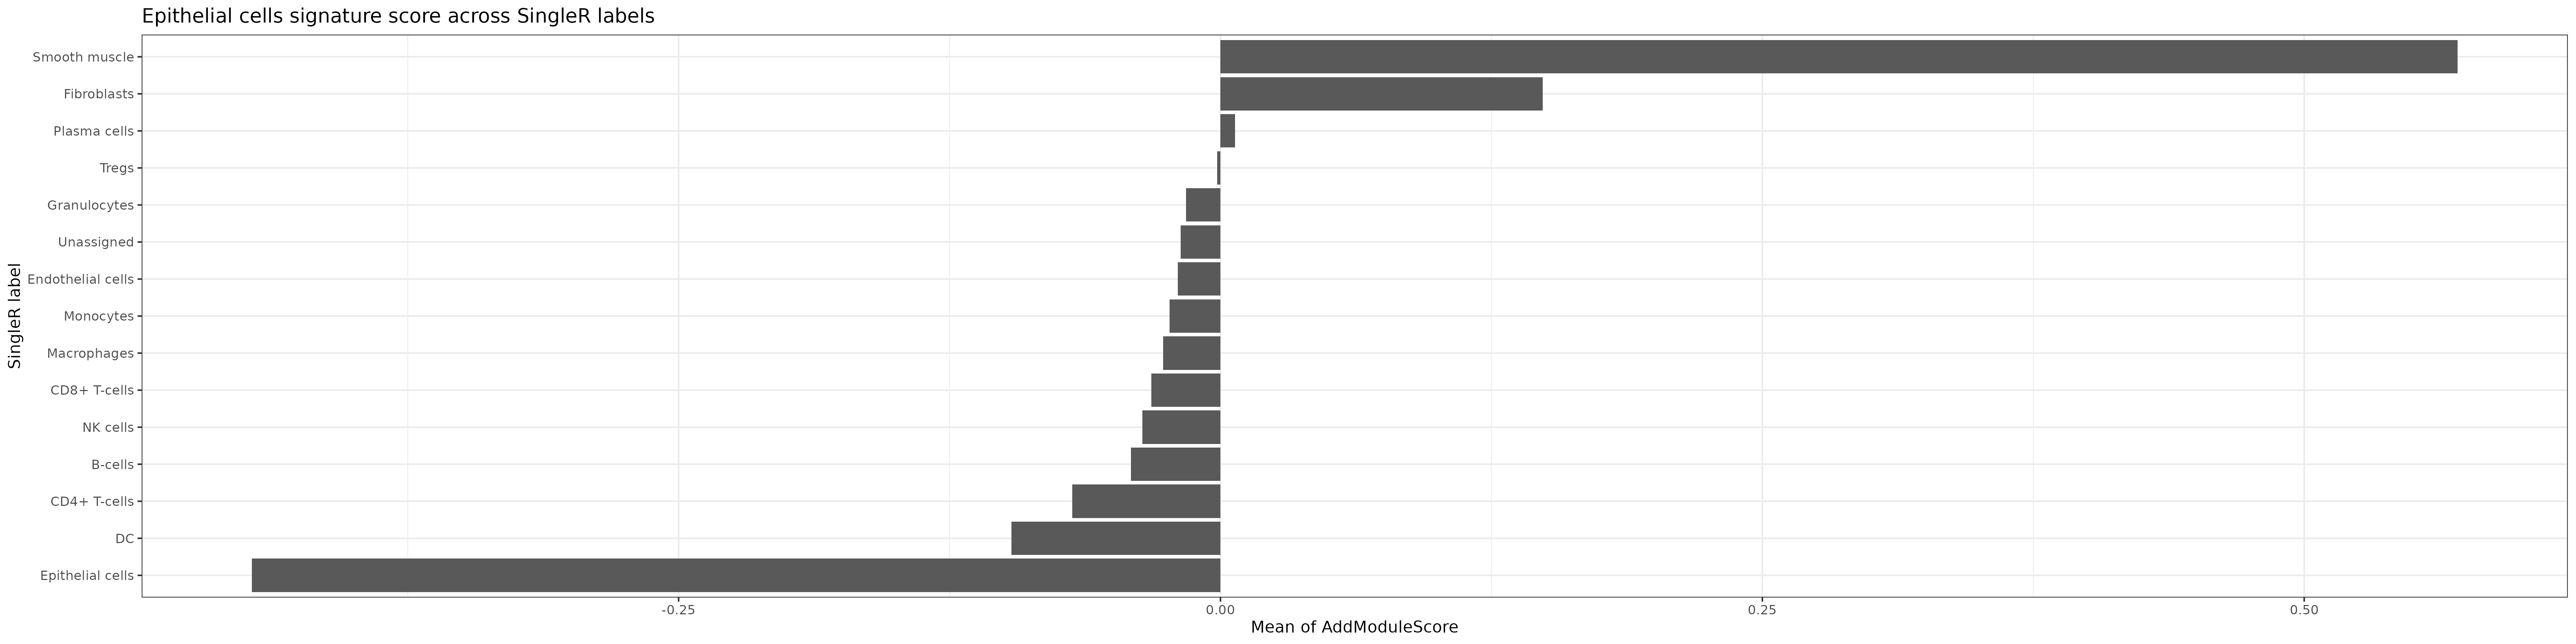
\includegraphics[width=\textwidth]{images/Epithelial_cells_Signature_BAD.png}
    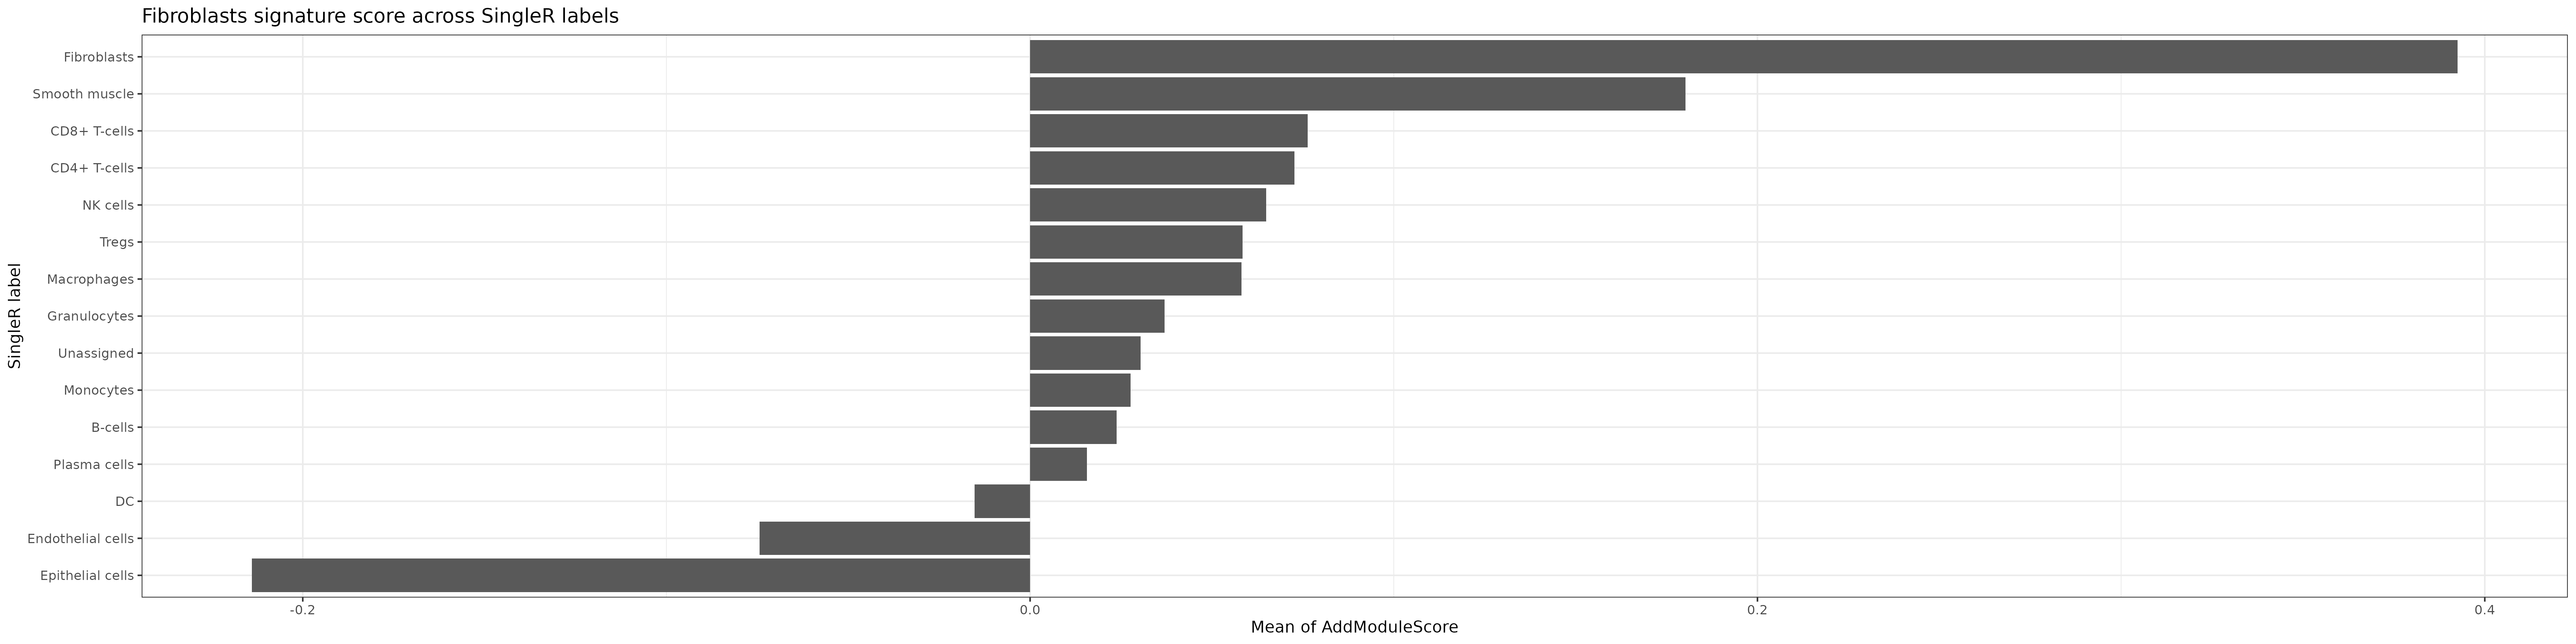
\includegraphics[width=\textwidth]{images/Fibroblasts_Signature.png}
    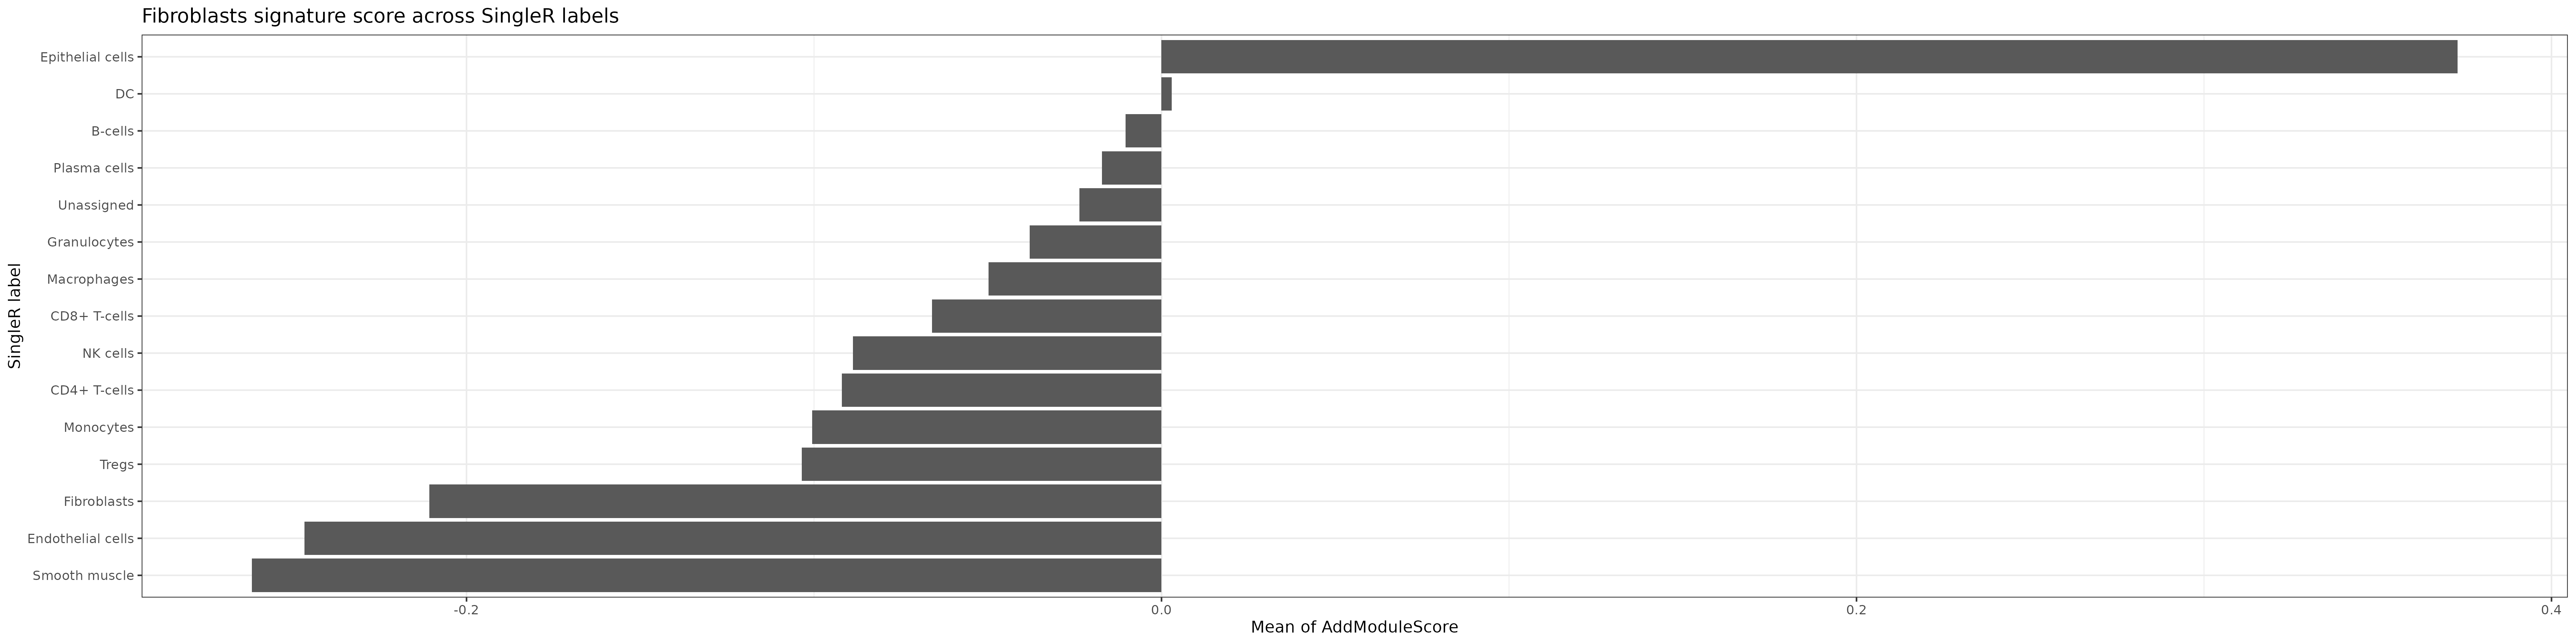
\includegraphics[width=\textwidth]{images/Fibroblasts_Signature_BAD.png}
    \caption{Effect of incorrect filtering using \(\lvert \log_2FC \rvert > 1\) in Epithelial and Fibroblasts signatures. Including negatively enriched genes introduced substantial bias into the enrichment signatures. Biased signatures still follow the canonical signatures of their corresponding cell types.}
    \labfig{AddModuleScoreBAD}
\end{figure} 

\textbf{Enrichment analysis} in transcriptomics is a computational approach used to identify biological themes, pathways, or cellular functions that are over-represented within a set of genes or proteins. Its purpose is to transform a long list of statistically significant genes into biologically meaningful insights by determining whether specific functional gene groups are enriched beyond what would be expected by chance. In the context of single-cell transcriptomics, enrichment analysis provides a continuous score for each individual cell, allowing the evaluation of whether a transcriptional signal is strong and coherent across a cell population or weak and dispersed.

This method consists of calculating, for each cell, the average expression of a predefined gene program and subtracting the aggregated expression of control gene sets used as background:
\[
\text{score} = \text{mean expression of target genes} - \text{mean expression of background genes}
\]
From the marker genes obtained through differential expression analysis, enrichment analysis was performed\sidenote{Using the \texttt{AddModuleScore} function from the \textbf{Seurat} package.} to evaluate whether each annotated cell type expressed its corresponding gene program more strongly than would be expected by random background expression. Consequently, every individual cell received a continuous enrichment score. A high score indicates that the transcriptional program associated with a given cell type is actively expressed above baseline background levels.

Unlike differential expression analysis, enrichment analysis does not perform a statistical comparison between groups of cells. Instead, it evaluates whether a biological program is active within each individual cell relative to a neutral background distribution. This allows the identification of coherent transcriptional signatures even in populations that may partially overlap at the gene-expression level.

\begin{figure}[H]
    \centering
    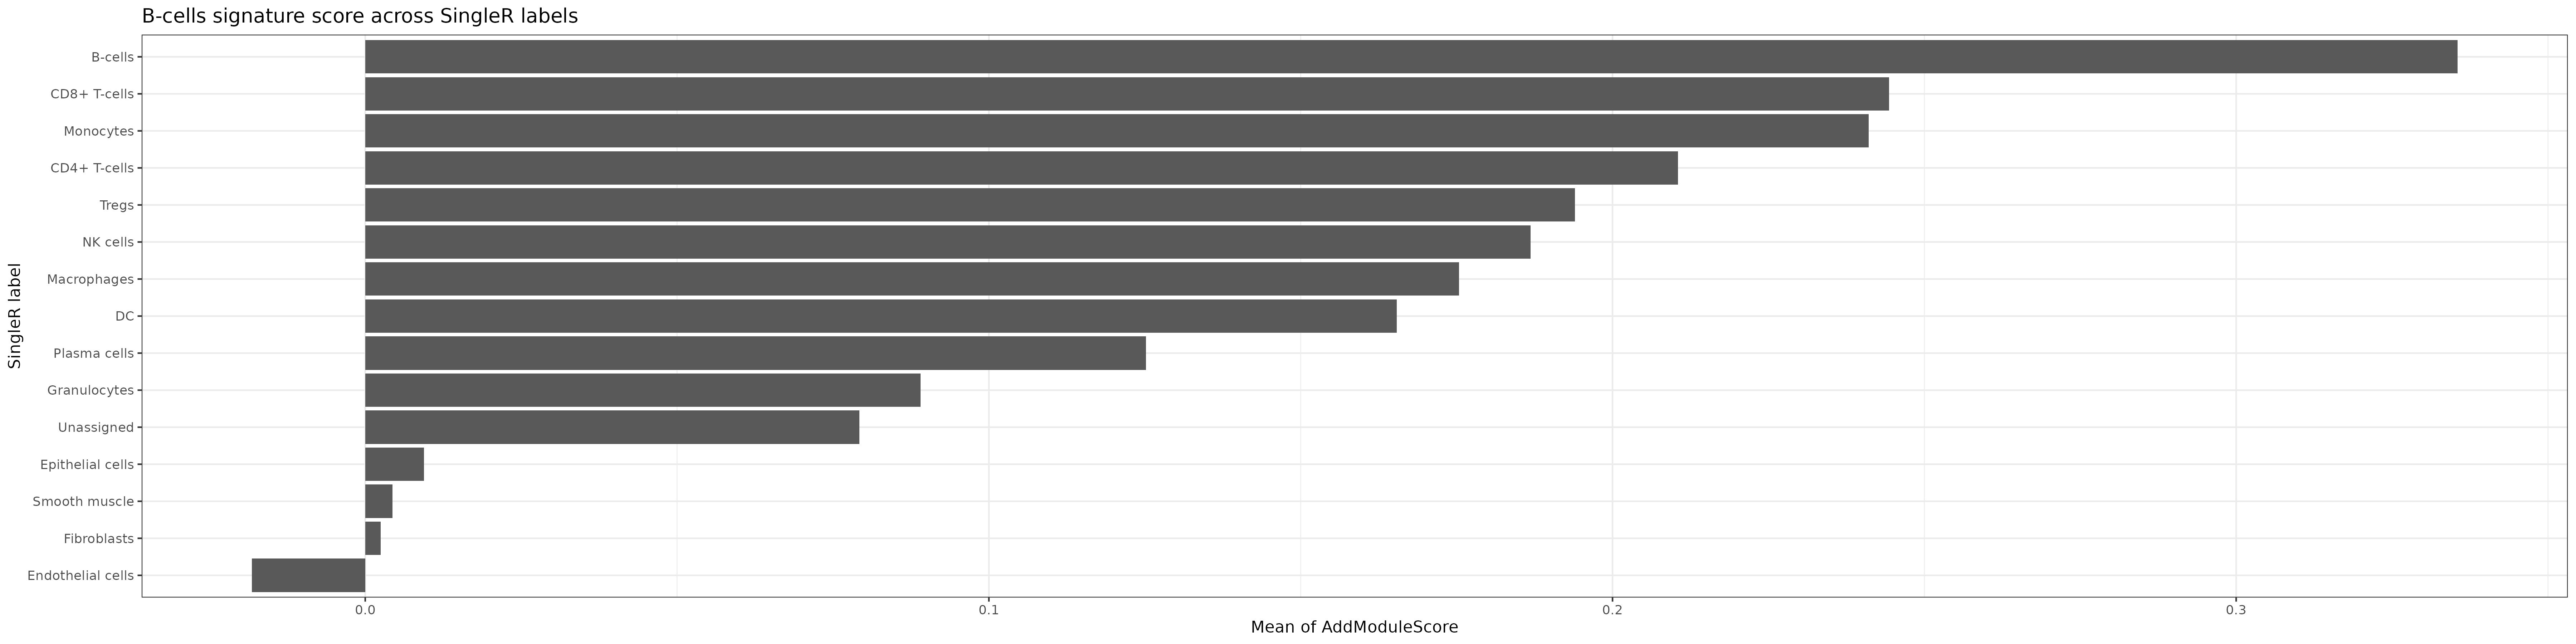
\includegraphics[width=\textwidth]{images/B-cells_Signature.png}
    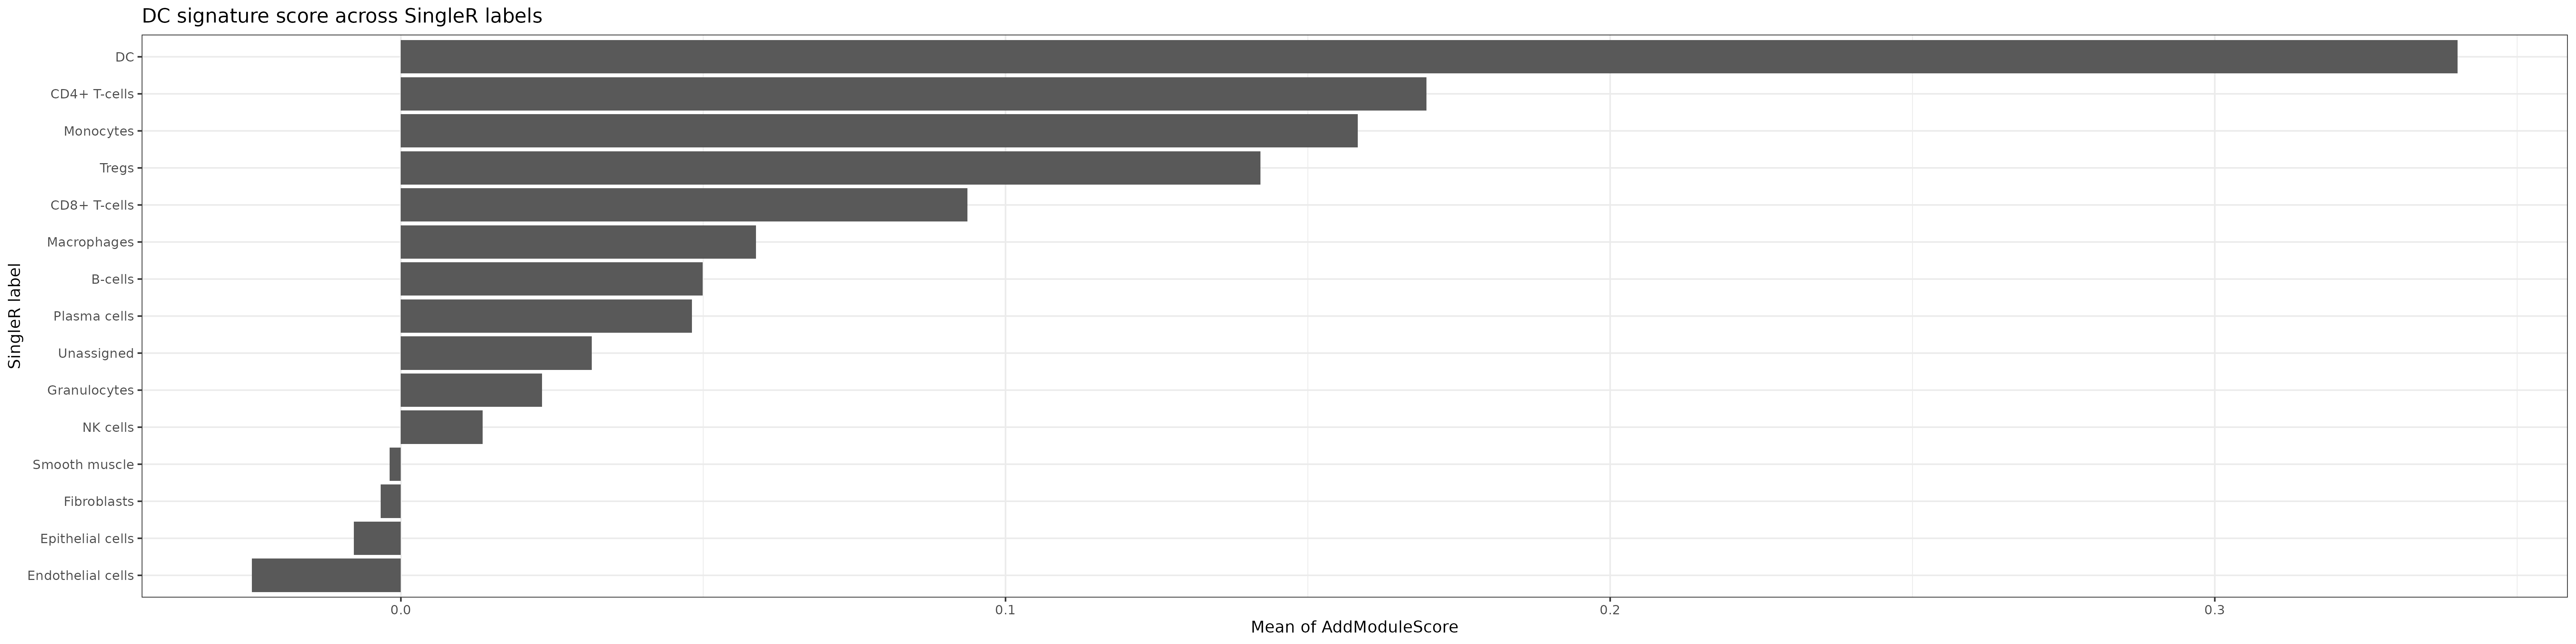
\includegraphics[width=\textwidth]{images/DC_Signature.png}
	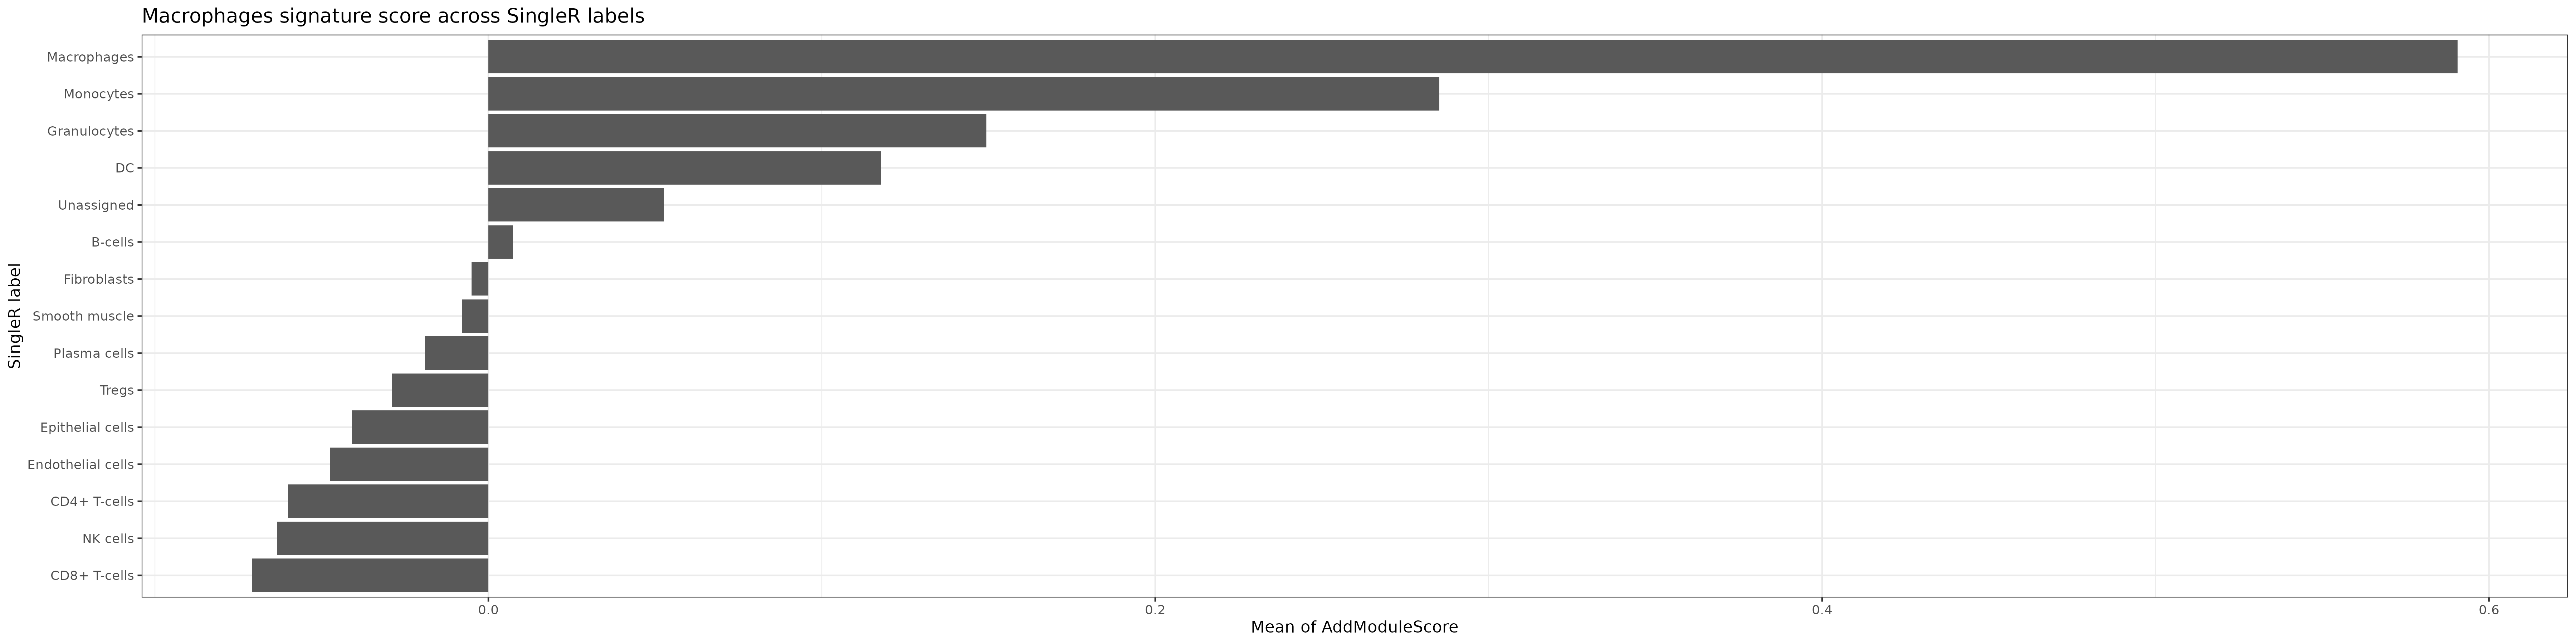
\includegraphics[width=\textwidth]{images/Macrophages_Signature.png}
	
\includegraphics[width=\textwidth]{images/Tregs_Signature.png}
	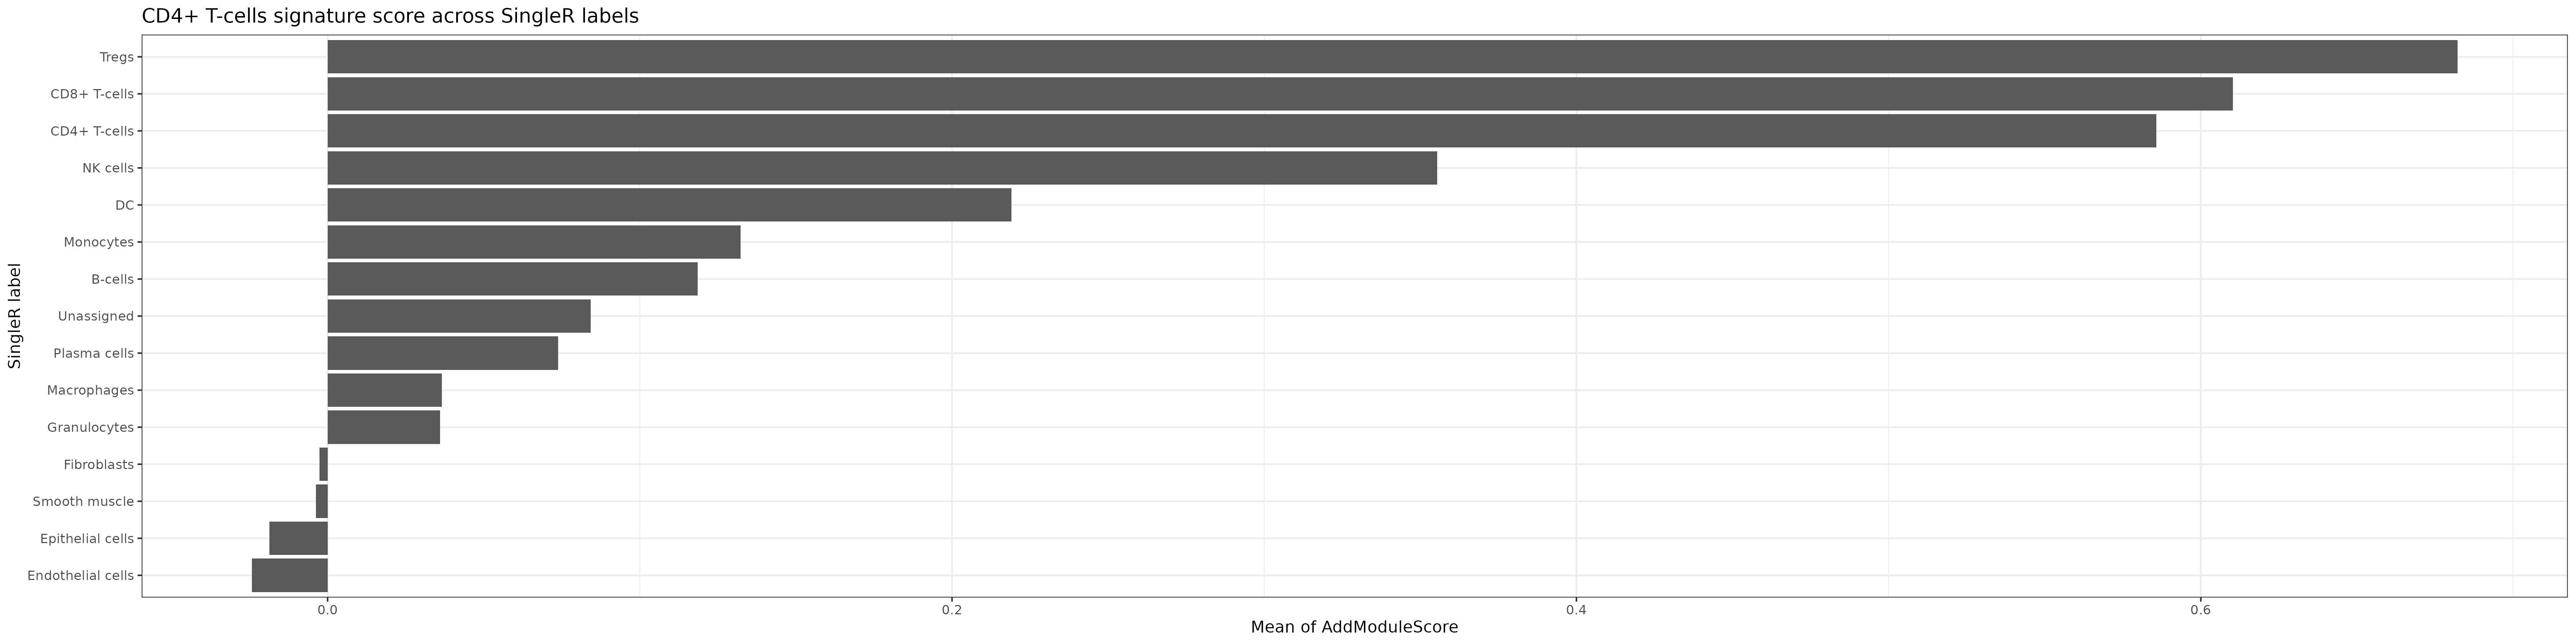
\includegraphics[width=\textwidth]{images/CD4+_T-cells_Signature.png}
	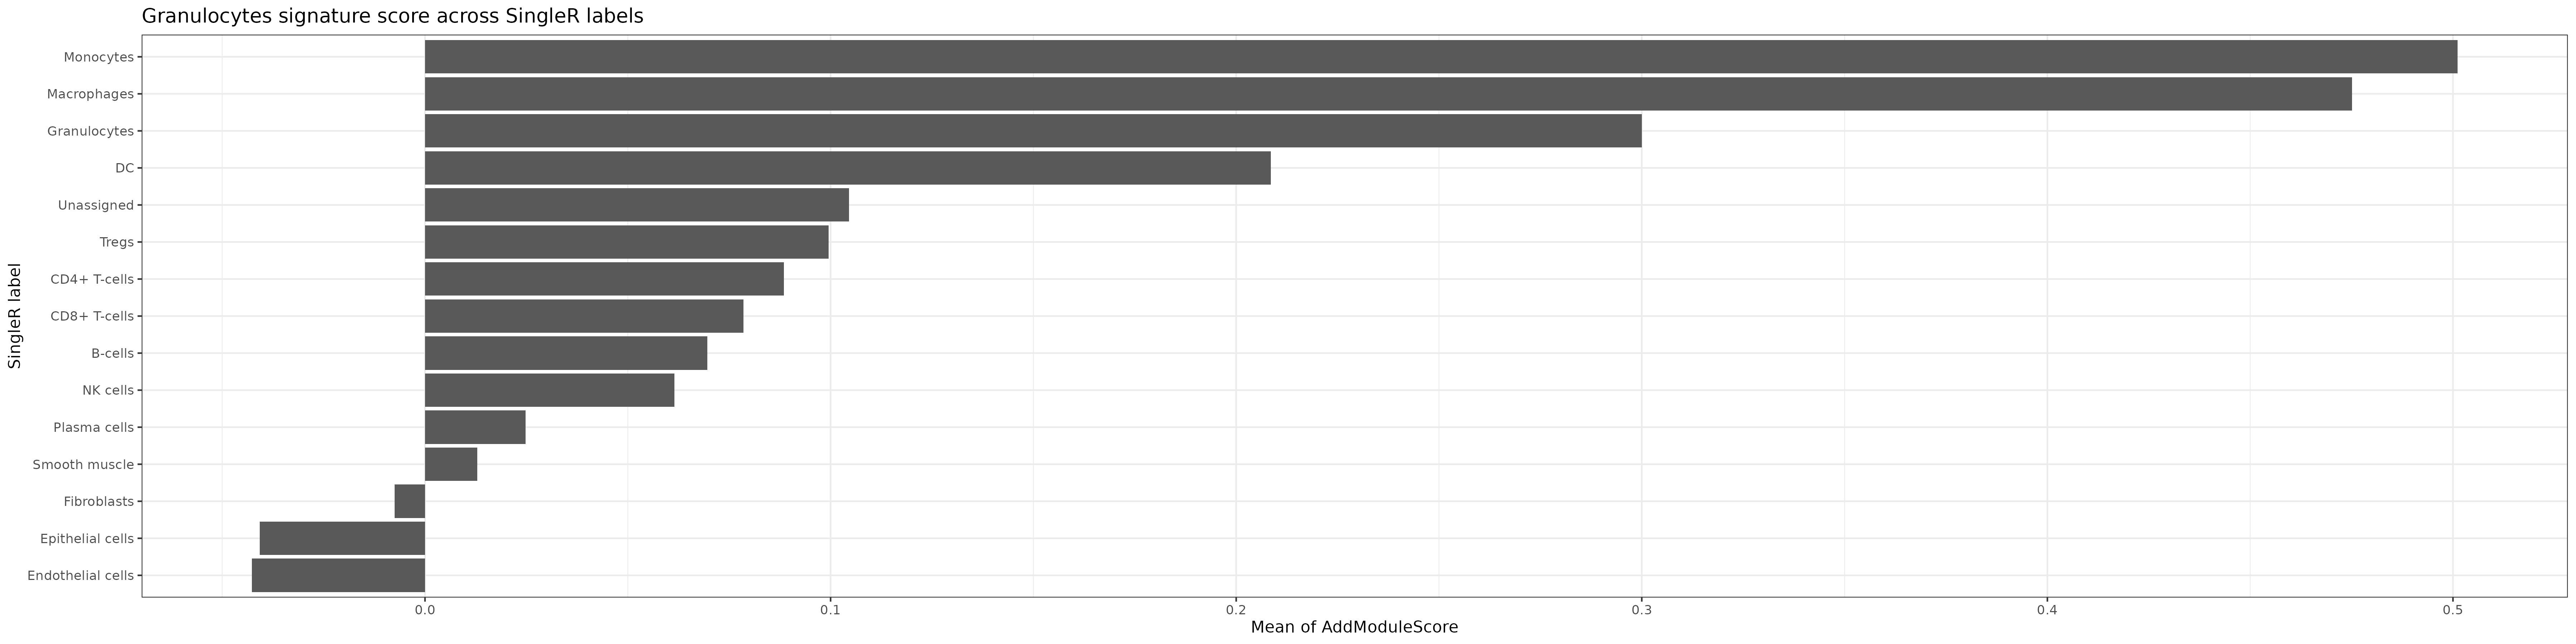
\includegraphics[width=\textwidth]{images/Granulocytes_Signature.png}
    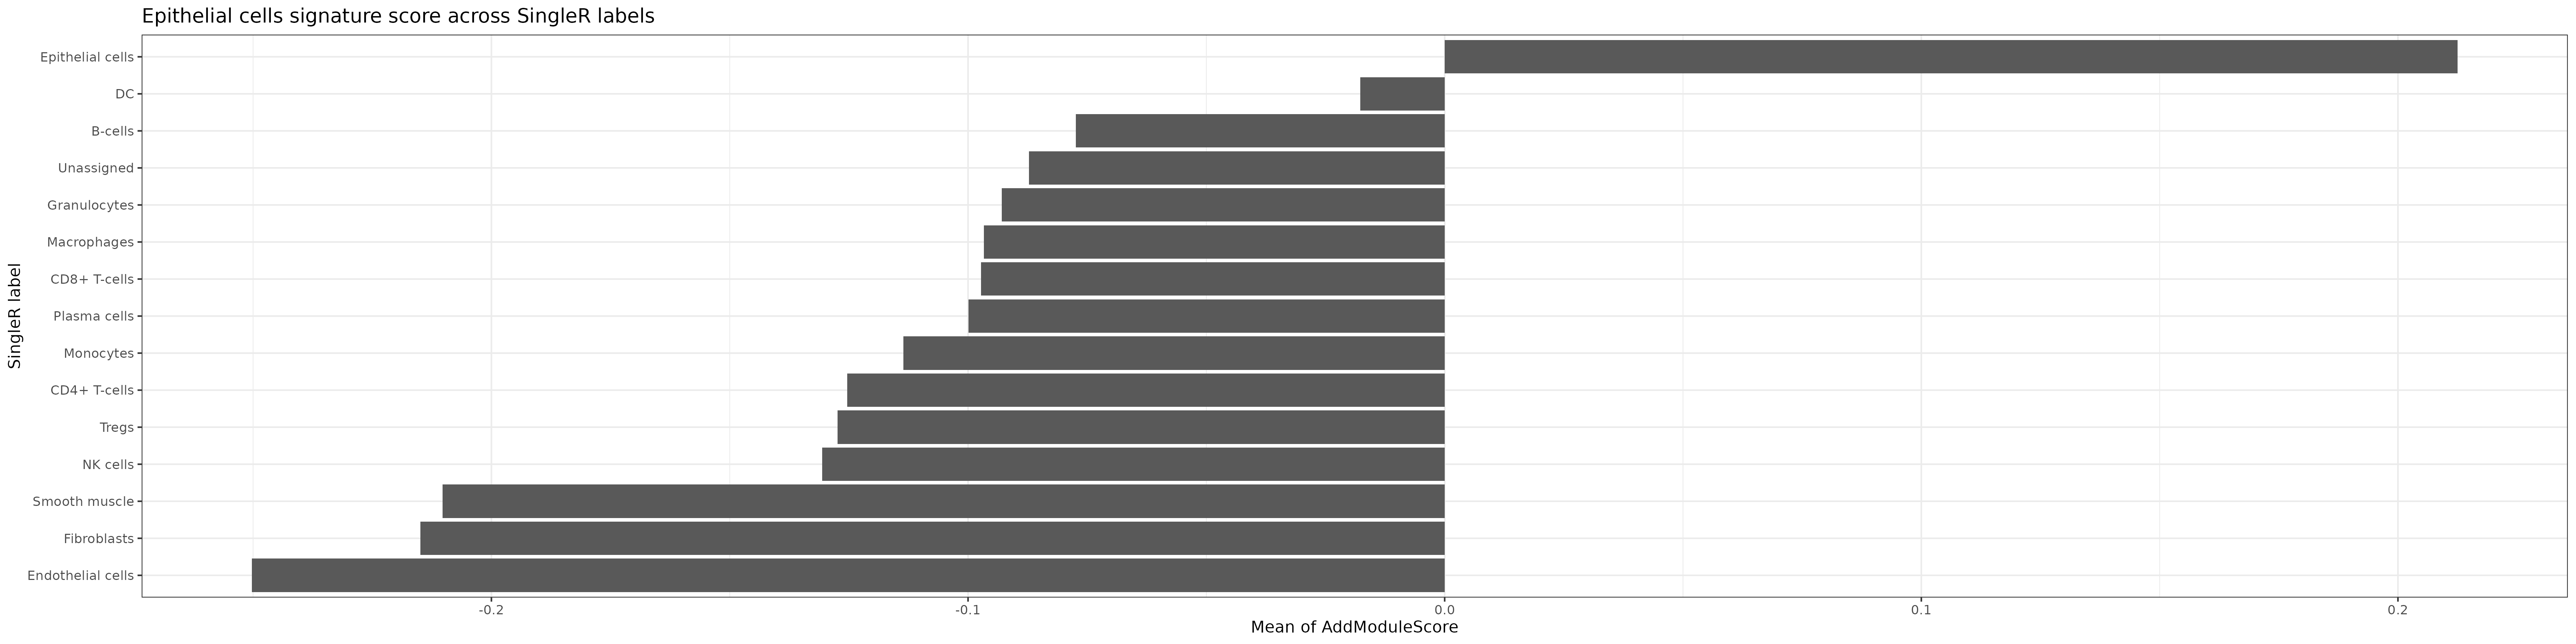
\includegraphics[width=\textwidth]{images/Epithelial_cells_Signature.png}
    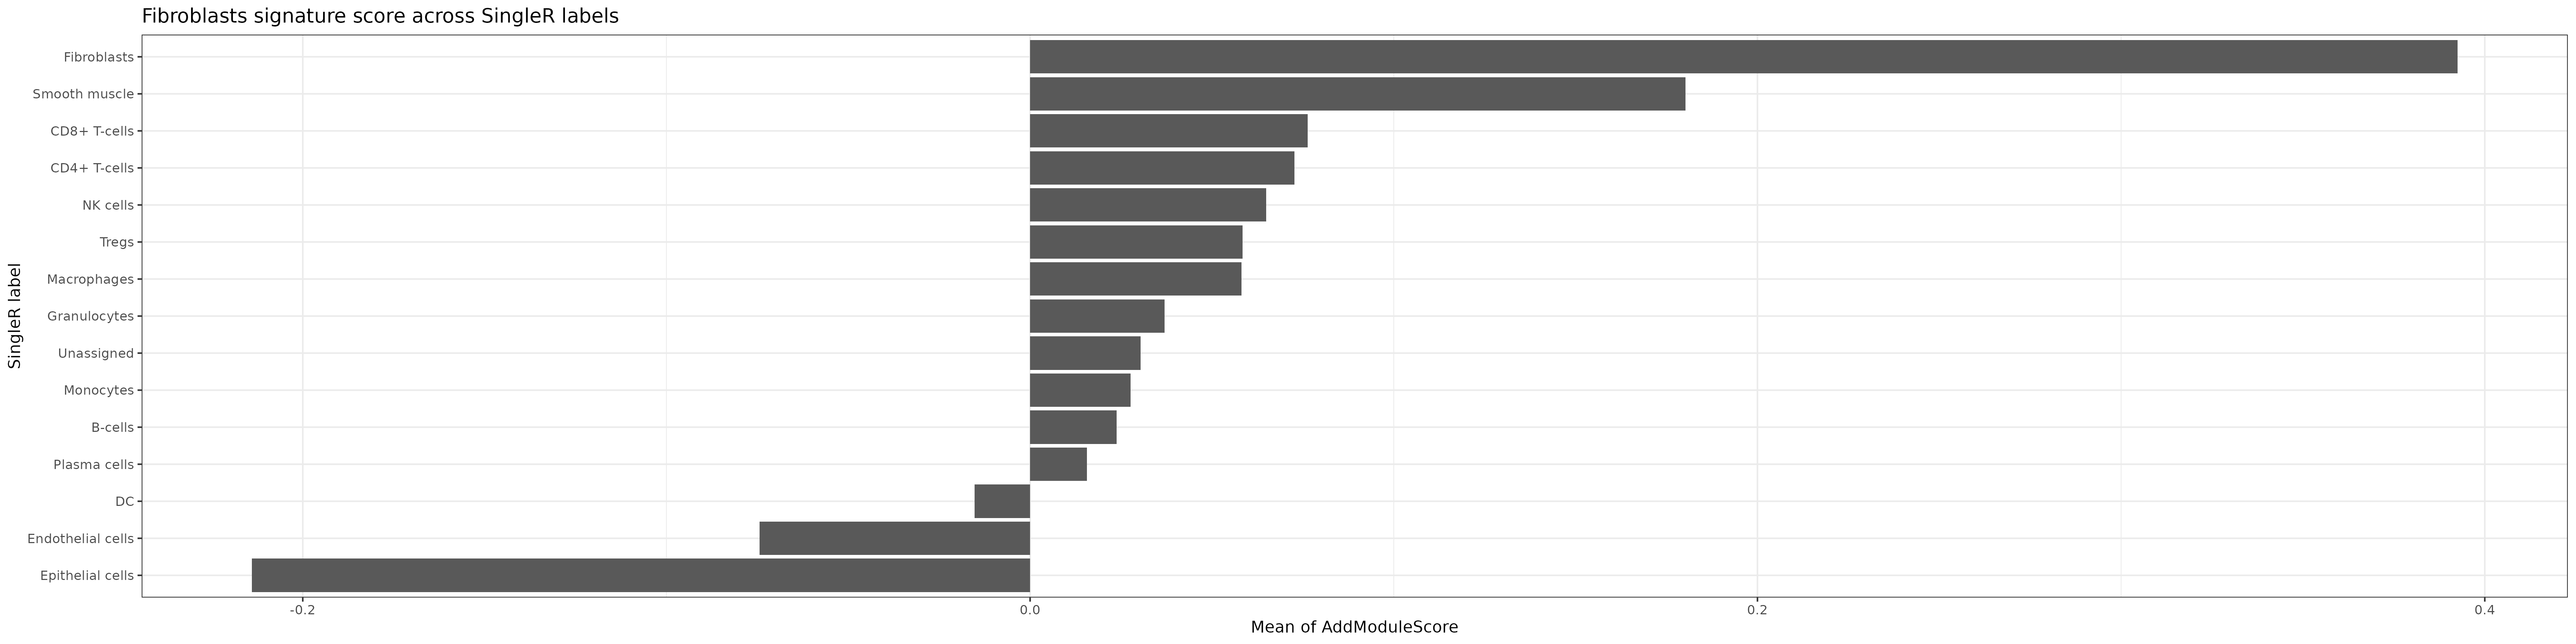
\includegraphics[width=\textwidth]{images/Fibroblasts_Signature.png}
    \caption{Module-score enrichment plots generated using the \textbf{mean} enrichment score obtained from \texttt{AddModuleScore}. Using the \textbf{sum} of enrichment scores would introduce a strong bias associated with the number of cells in each cluster. Without standardisation of the score, highly abundant populations would artificially display stronger signatures due to cluster size rather than true biological enrichment.}
    \labfig{AddModuleScore}
\end{figure}


The additional validation step focused on cell types that showed ambiguous enrichment patterns after the initial marker-based analysis. Importantly, this ambiguity was interpreted carefully because overlapping module scores do not necessarily indicate incorrect annotation. In many cases, they reflect biologically expected similarities between related cell populations. For example, granulocytes in both \reffig{Dotplot} and \reffig{AddModuleScore} showed partial similarity with monocytes and macrophages. This behaviour was considered biologically consistent with their shared myeloid origin and their common involvement in innate immune and inflammatory responses. Therefore, the overlap was not interpreted as evidence of misclassification, but rather as an expected relationship between related myeloid populations. The same reasoning was applied to CD4+ T cells, which showed partial similarity with CD8+ T cells\sidenote{This population was included as an explanatory example despite not displaying the highest CD4 enrichment score within the expected cluster, since the observed close overlap still remained biologically consistent with the expected transcriptional behaviour of closely related T-cell populations.} and Tregs. This overlap is biologically expected because these populations share a common T-cell transcriptional background. However, the dot plot provided additional clarification of the annotation: CD4+ T cells did not show clear expression of CD8 markers or FOXP3, which are canonical markers of CD8+ T cells and Tregs, respectively. This supported the interpretation that the CD4+ T-cell annotation remained biologically valid despite the partial overlap observed in the module-score distributions. 

According to the automatic validation criterion implemented in this pipeline, these populations were flagged as ambiguous because the highest enrichment score of the corresponding signature was not observed in the expected annotation label. However, this result was not interpreted as direct evidence of incorrect annotation. Instead, it suggested that the signatures derived from the global differential expression analysis were not sufficiently specific to fully represent these populations in the current sample. Consequently, these groups were considered biologically ambiguous populations requiring further inspection rather than being automatically reassigned.


The purpose of the subsequent subset analysis was not to repeat the complete annotation process, but rather to obtain markers that were more specific for the populations that remained uncertain. In the global differential expression analysis\sidenote{Performed using the \texttt{FindAllMarkers} function from the \textbf{Seurat} package.}, each cell type was compared against all remaining cells in the dataset. Although this strategy is effective for broad annotation, it may fail to identify highly discriminative markers for closely related populations. By restricting the differential expression analysis to the uncertain labels only, the comparison became more specific and allowed more discriminative markers to emerge.

After performing the subset-based differential expression analysis, characteristic markers for each population became more evident, including canonical markers that were less clearly detected in the global comparison. In addition, direct pairwise comparisons\sidenote{Performed using the \texttt{FindMarkers} function from the \textbf{Seurat} package.} demonstrated that the candidate populations maintained clearly distinct transcriptional profiles. These results supported the interpretation that the observed overlap did not arise from annotation errors, but rather from biologically related populations requiring more specific comparisons for proper validation.

\begin{marginfigure}
	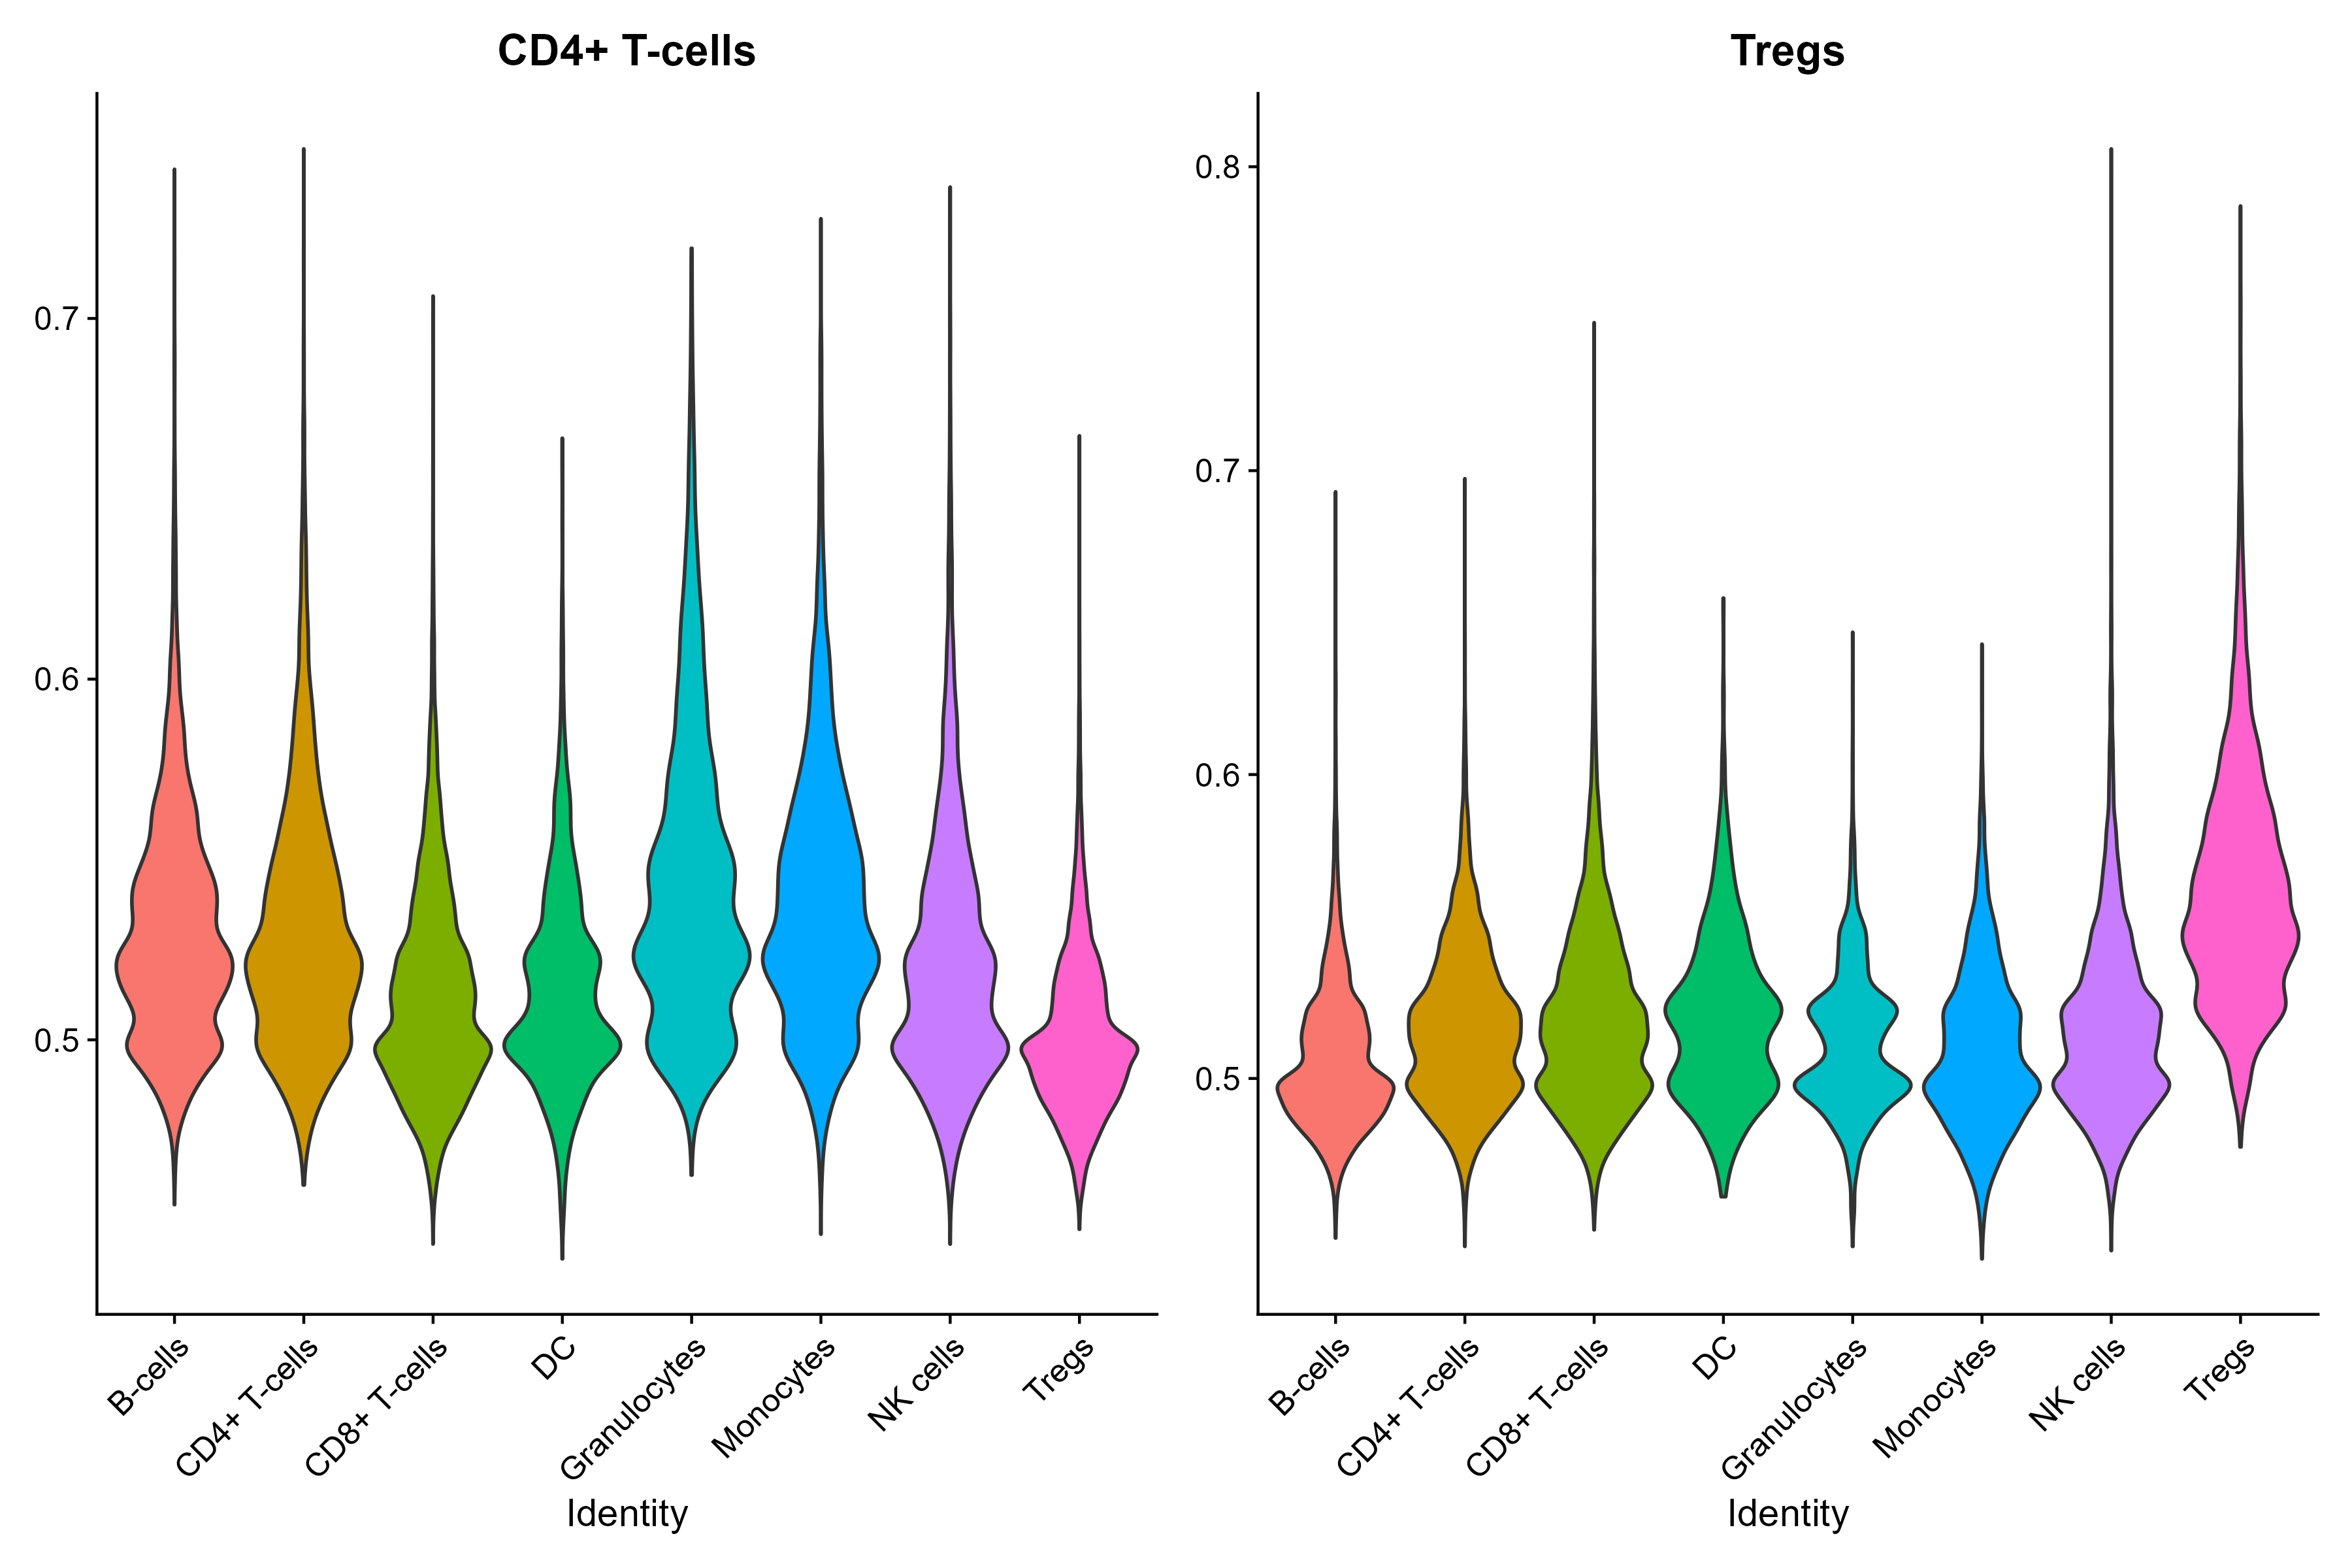
\includegraphics{images/CD4+ T-cells_Tregs_Violin_plot.png}
    \caption{Example of violin-plot validation. Fortunately, no sample in the final dataset required this final validation layer. Therefore, a representative example was generated to illustrate how violin plots can be used as an additional validation strategy. In this example, the expression distributions of canonical CD4 and Treg markers clearly differ between populations, supporting their separation despite partial overlap in previous enrichment analyses.}
\end{marginfigure}

Finally, violin plots were used as a last inspection step for the most uncertain comparisons. These plots enabled the visualisation of selected marker or signature expression distributions across candidate populations. While module scores provided a global summary of transcriptional-program enrichment, violin plots allowed direct inspection of whether the relevant markers were concentrated within the expected population and reduced in alternative populations. Therefore, the combination of global marker detection, module-score validation, targeted subset analysis, and violin-plot inspection provided a stepwise validation strategy capable of distinguishing true biological overlap from potential annotation uncertainty.

In summary, the annotation strategy implemented in this workflow combined supervised reference-based classification with multiple complementary validation layers in order to maximise biological reliability while minimising annotation bias. Although SingleR provided an efficient first approximation of cell identities, the subsequent integration of differential expression analysis, enrichment analysis, subset-based comparisons, and violin-plot inspection demonstrated that accurate annotation in single-cell transcriptomics cannot rely exclusively on automated classification methods. The results showed that transcriptional overlap between biologically related populations is common and does not necessarily indicate misclassification, particularly in immune populations sharing developmental origins or functional programs. Furthermore, this workflow highlighted the importance of carefully selecting statistical filters and validation criteria, as inappropriate thresholds can introduce substantial biological bias into downstream analyses. Overall, the combination of global and targeted validation approaches provided a robust framework for distinguishing true biological similarity from potential annotation uncertainty, leading to a more reliable characterisation of the cellular composition of bladder tumour samples.

%%%%%%%%%%%%%%%%%%%%%%%%%%%%%%%%%%%%%%%%%%%%%%%%%%%%%%%%%%%%%%%%%%%%%%%%%%%%%%%%%%%%%%%%%%%%%%%
% Sidenotes are a distinctive feature of all 1.5-column-layout books. 
% Indeed, having wide margins means that some material can be displayed 
% there. We use margins for all kind of stuff: sidenotes, marginnotes, 
% small tables of contents, citations, and, why not?, special boxes and 
% environments.

% \section{Sidenotes}

% Sidenotes are like footnotes, except that they go in the margin, where 
% they are more readable. To insert a sidenote, just use the command 
% \Command{sidenote\{Text of the note\}}. You can specify a 
% mark\sidenote[O]{This sidenote has a special mark, a big O!} with \\ 
% \Command{sidenote[mark]\{Text\}}, but you can also specify an offset, 
% which moves the sidenote upwards or downwards, so that the full syntax is:

% \begin{lstlisting}[style=kaolstplain]
% \sidenote[mark][offset]{Text}
% \end{lstlisting}

% If you use an offset, you always have to add the brackets for the mark, 
% but they can be empty.\sidenote{If you want to know more about the usage 
% of the \Command{sidenote} command, read the documentation of the 
% \Package{sidenotes} package.}

% In \Class{kaobook} we copied a feature from the \Package{snotez} 
% package: the possibility to specify a multiple of \Command{baselineskip} 
% as an offset. For example, if you want to enter a sidenote with the 
% normal mark and move it upwards one line, type:

% \begin{lstlisting}[style=kaolstplain]
% \sidenote[][*-1]{Text of the sidenote.}
% \end{lstlisting}

% As we said, sidenotes are handled through the \Package{sidenotes} 
% package, which in turn relies on the \Package{marginnote} package.

% \section{Marginnotes}

% This command is very similar to the previous one. You can create a 
% marginnote with \Command{marginnote[offset]\{Text\}}, where the offset 
% argument can be left out, or it can be a multiple of 
% \Command{baselineskip},\marginnote[-1cm]{While the command for margin 
% notes comes from the \Package{marginnote} package, it has been redefined 
% in order to change the position of the optional offset argument, which 
% now precedes the text of the note, whereas in the original version it 
% was at the end. We have also added the possibility to use a multiple of 
% \Command{baselineskip} as offset. These things were made only to make 
% everything more consistent, so that you have to remember less things!} 
% \eg

% \begin{lstlisting}[style=kaolstplain]
% \marginnote[-12pt]{Text} or \marginnote[*-3]{Text}
% \end{lstlisting}

% \begin{kaobox}[frametitle=To Do]
% A small thing that needs to be done is to renew the \Command{sidenote} 
% command so that it takes only one optional argument, the offset. The 
% special mark argument can go somewhere else. In other words, we want the 
% syntax of \Command{sidenote} to resemble that of \Command{marginnote}.
% \end{kaobox}

% We load the packages \Package{marginnote}, \Package{marginfix} and 
% \Package{placeins}. Since \Package{sidenotes} uses \Package{marginnote}, 
% what we said for marginnotes is also valid for sidenotes. Side- and 
% margin- notes are shifted slightly upwards 
% (\Command{renewcommand\{\textbackslash marginnotevadjust\}\{3pt\}}) in 
% order to align them to the bottom of the line of text where the note is 
% issued. Importantly, both sidenotes and marginnotes are defined as 
% floating if the optional argument (\ie the vertical offset) is left 
% blank, but if the offset is specified they are not floating. Recall that 
% floats cannot be nested, so in some rare cases you may encounter errors 
% about lost floats; in those cases, remember that sidenotes and 
% marginnotes are floats. To solve the problem, it may be possible to 
% transform them into non-floating elements by specifying an offset of 
% 0pt.

% \section{Footnotes}

% Even though they are not displayed in the margin, we will discuss about 
% footnotes here, since sidenotes are mainly intended to be a replacement 
% of them. Footnotes force the reader to constantly move from one area of 
% the page to the other. Arguably, marginnotes solve this issue, so you 
% should not use footnotes. Nevertheless, for completeness, we have left 
% the standard command \Command{footnote}, just in case you want to put a 
% footnote once in a while.\footnote{And this is how they look like. 
% Notice that in the PDF file there is a back reference to the text; 
% pretty cool, uh?}

% \section{Margintoc}

% Since we are talking about margins, we introduce here the 
% \Command{margintoc} command, which allows one to put small table of 
% contents in the margin. Like other commands we have discussed, 
% \Command{margintoc} accepts a parameter for the vertical offset, like 
% so: \Command{margintoc[offset]}.

% The command can be used in any point of the document, but we think it 
% makes sense to use it just at the beginning of chapters or parts. In 
% this document I make use of a \KOMAScript\xspace feature and put it in 
% the chapter preamble, with the following code:

% \marginnote{The font used in the margintoc is the same as the one for 
% 	the chapter entries in the main table of contents at the beginning 
% 	of the document.}

% \begin{lstlisting}[style=kaolstplain]
% \setchapterpreamble[u]{\margintoc}
% \chapter{Chapter title}
% \end{lstlisting}

% As the space in the margin is a valuable resource, there is the 
% possibility to print a shorter version of the title in the margin toc. 
% Thus, there are in total three possible versions for the title of a 
% section (or subsection): the one for the main text, the one for the main 
% table of contents, and the one for the margintoc. These versions can be 
% specified at the same time when the section is created in the source 
% \TeX file:
% \begin{lstlisting}[style=kaolstplain]
% \section[alternative-title-for-toc]{title-as-written-in-text}[alternative-title-for-margintoc]
% \end{lstlisting}

% By default, the margintoc includes sections and subsections.
% If you only want to show sections, add
% \begin{lstlisting}[style=kaolstplain]
% \setcounter{margintocdepth}{\sectiontocdepth}
% \end{lstlisting}
% somewhere in your preamble.

% \section{Marginlisting}

% On some occasions it may happen that you have a very short piece of code 
% that doesn't look good in the body of the text because it breaks the 
% flow of narration: for that occasions, you can use a 
% \Environment{marginlisting}. The support for this feature is still 
% limited, especially for the captions, but you can try the following 
% code:

% \begin{marginlisting}[-1.35cm]
% 	\caption{An example of a margin listing.}
% 	\vspace{0.6cm}
% 	\begin{lstlisting}[language=Python,style=kaolstplain]
% print("Hello World!")
% 	\end{lstlisting}
% \end{marginlisting}

% \begin{verbatim}
% \begin{marginlisting}[-0.5cm]
% 	\caption{My caption}
% 	\vspace{0.2cm}
% 	\begin{lstlisting}[language=Python,style=kaolstplain]
% 	... code ...
% 	\end{lstlisting}
% \end{marginlisting}
% \end{verbatim}

% Unfortunately, the space between the caption and the listing must be 
% adjusted manually; if you find a better way, please let me know.

% Not only textual stuff can be displayed in the margin, but also figures. 
% Those will be the focus of the next chapter.
